\documentclass{article}
\usepackage{graphicx} 

\title{Abgabe 1 für Computergestützte Methoden}
\author{Gruppe 69, Toni und Enver }
\date{02.12.2024}





\usepackage[utf8]{inputenc}
\usepackage[T1]{fontenc}
\usepackage[ngerman]{babel}
\usepackage[margin=1in]{geometry} 
\usepackage{hyperref}
\usepackage{amsmath}
\usepackage{graphicx}
\usepackage{parskip} 
\usepackage{xcolor}
\usepackage{longtable}


\newcommand{\redboxlink}[2]{\textsuperscript{\hyperlink{#1}{\fbox{\textcolor{red}{#2}}}}}


\newcommand{\greenboxlink}[2]{\hyperlink{#1}{\fbox{\textcolor{green}{#2}}}}


\title{Abgabe 1 für Computergestützte Methoden}
\author{Gruppe 69; Enver Özer Demir(MatrNu.: 4337179),
Toni Tornede(MatrNu.:4352117)}
\date{02.12.2024}

\begin{document}


\maketitle
\tableofcontents
\newpage


\section{Der zentrale Grenzwertsatz}
\label{sec:zgs}

Der zentrale Grenzwertsatz (ZGS) ist ein fundamentales Resultat der Wahrscheinlichkeitstheorie, das die Verteilung von Summen unabhängiger, identisch verteilter (i.i.d.) Zufallsvariablen (ZV) beschreibt. Er besagt, dass unter bestimmten Voraussetzungen die Summe einer großen Anzahl solcher ZV annähernd normalverteilt ist, unabhängig von der Verteilung der einzelnen ZV. Dies ist besonders nützlich, da die Normalverteilung gut untersucht und mathematisch handhabbar ist.

\subsection{Aussage}
Sei $X_1, X_2, \dots, X_n$ eine Folge von i.i.d. Zufallsvariablen mit dem Erwartungswert $\mu = E(X_i)$ und der Varianz $\sigma^2 = \text{Var}(X_i)$, wobei $0 < \sigma^2 < \infty$ gilt. Dann konvergiert die standardisierte Summe $Z_n$ dieser Zufallsvariablen für $n \to \infty$ in Verteilung gegen eine \textbf{Standardnormalverteilung:}\redboxlink{zgs1}{1} 
\begin{equation}
Z_n = \frac{\sum_{i=1}^n X_i - n\mu}{\sigma \sqrt{n}} \overset{d}{\to} N(0,1). \tag{1}
\end{equation}
Das bedeutet, dass für große $n$ die Summe der Zufallsvariablen näherungsweise normalverteilt ist mit Erwartungswert $n\mu$ und Varianz $n\sigma^2$:
\begin{equation}
\sum_{i=1}^n X_i \sim N(n\mu, n\sigma^2). \tag{2}
\end{equation}

\subsection{Erklärung der Standardisierung}
\label{zgs1}
Um die Summe der Zufallsvariablen in eine Standardnormalverteilung zu transformieren, subtrahiert man den Erwartungswert $n\mu$ und teilt durch die Standardabweichung $\sigma \sqrt{n}$. Dies führt zu der \textbf{obigen Formel} \hyperlink{zgs1}{\fbox{\textcolor{red}{(1)}}}. Die \textbf{Darstellung} \hyperlink{zgs2}{\fbox{\textcolor{red}{(2)}}} ist für $n \to \infty$ nicht wohldefiniert.

\subsection{Anwendungen}
\begin{itemize}
    \item \textbf{Würfeln mit einem fairen Würfel}: Wenn man viele Stichproben der Mittelwerte von 10 Würfen eines fairen Würfels berechnet, nähern sich die Mittelwerte einer Normalverteilung an.
    \item \textbf{Münzwürfe}: Der Anteil von "Kopf" in großen Stichproben aus Münzwürfen folgt einer Normalverteilung, auch wenn die Einzelereignisse binomial verteilt sind.
\end{itemize}

\footnotetext[1]{\hypertarget{litref}{Der zentrale Grenzwertsatz hat verschiedene Verallgemeinerungen. Eine davon ist der \textbf{Lindeberg-Feller-Zentrale-Grenzwertsatzes} [\greenboxlink{litref}{[1]}, Seite 328], der schwächere Bedingungen an die Unabhängigkeit und die identische Verteilung der ZV stellt.}}

\newpage 


\section{Bearbeitung zur Aufgabe 1}
\label{sec:aufgabe1}

\subsection{Datenverarbeitung}
\label{sec:datenverarbeitung}

Die Untersuchung der Daten für Gruppe 69 ergab, dass der Datensatz eine Vielzahl von Attributen enthält, die sowohl zeitliche als auch meteorologische Informationen umfassen. Die Daten erstrecken sich über den Zeitraum vom 01.01.2023 bis zum 31.12.2023 und beziehen sich auf die Station „North Moore St \& Greenwich St“. Jede Gruppe enthält 365 Einträge, die ein Jahr abbilden. 

\textbf{Struktur der Daten:}
Der Datensatz besteht aus den folgenden Spalten:
\begin{itemize}
    \item \textbf{Group}: Gruppenzuordnung (Werte: {1, 2, ..., 100}).
    \item \textbf{Station}: Stationsnamen, z. B. „North Moore St \& Greenwich St“.
    \item \textbf{Date}: Datum im Format JJJJ-MM-TT.
    \item \textbf{Day\_of\_year}: Nummer des Tages im Jahr (1–365).
    \item \textbf{Day\_of\_week}: Wochentag (1 = Montag, 7 = Sonntag).
    \item \textbf{Month\_of\_year}: Monat des Jahres (1 = Januar, ..., 12 = Dezember).
    \item \textbf{Precipitation}: Niederschlag (z. B. in Zoll, mit Platzhaltern -1 oder NA für fehlende Werte).
    \item \textbf{Windspeed}: Windgeschwindigkeit in mph (ebenfalls mit -1 oder NA für fehlende Werte).
    \item \textbf{Min\-temperature, Average\-temperature, Max\-temperature}: Temperaturen in Fahrenheit.
    \item \textbf{Count}: Anzahl der verliehenen Fahrräder.
\end{itemize}

Die Daten zeigen, dass für Station „North Moore St \& Greenwich St“ (Gruppe 69) folgende Werte relevant sind:
\begin{itemize}
    \item Temperaturen variieren zwischen 4°F und 93°F.
    \item Niederschlagswerte reichen von -1 bis 8.05 Zoll (Platzhalter -1 für fehlende Werte).
    \item Windgeschwindigkeit liegt zwischen -1 und 21.47 mph.
    \item Die Anzahl der Fahrradausleihen liegt zwischen 1 und 707 pro Tag.
\end{itemize}

\textbf{Erste Erkenntnisse:}
- Die Daten weisen fehlende oder ungültige Werte (-1 oder NA) auf, die bei weiteren Analysen berücksichtigt werden müssen. 
- Es besteht eine starke zeitliche Struktur, da die Spalten „Date“, „Day\_of\_year“, „Day\_of\_week“ und „Month\_of\_year“ alle korrelieren.

\textbf{Potential für weitere Analysen:}
Die Daten bieten eine Grundlage für mehrere Forschungsfragen, wie z. B.:
\begin{itemize}
    \item Wie beeinflussen Wetterfaktoren wie Windgeschwindigkeit und Niederschlag die Fahrradausleihe?
    \item Welche Stationen oder Gruppen zeigen besonders hohe oder niedrige Ausleihzahlen?
    \item Wie stark variieren die Wetterbedingungen innerhalb eines Jahres an der Station von Gruppe 69?
\end{itemize}

\newpage 

\subsection{Tabellenkalkulation}
\label{sec:tabellenkalkulation}


Zuerst wurde die CSV-Datei in der Tabellenkalkulationssoftware Excel geladen. Da die Datei als CSV vorlag, wurde als Trennzeichen das Komma verwendet. Zusätzlich wurden Textbegrenzer wie Anführungszeichen berücksichtigt.

Die Spalten wurden auf korrekte Datentypen überprüft:
\begin{itemize}
    \item \textbf{Numerische Werte} (z. B. Count, Precipitation, Windspeed): Wurden als Zahlen erkannt.
    \item \textbf{Datumsspalten} (z. B. Date): Automatisch in Datumsformate konvertiert.
    \item \textbf{Textspalten} (z. B. Station): Blieben unverändert.
\end{itemize}

Mithilfe der Filterfunktion wurde die Bedingung „Group = 69“ angewandt, sodass nur die Daten dieser Gruppe angezeigt wurden. Es wurde sichergestellt, dass die ausgewählten Daten ausschließlich die Station „North Moore St \& Greenwich St“ umfassen, da wir mit den uns zugeteilten Daten arbeiten mussten.

Zuletzt ist noch wichtig zu erwähnen, dass die Werte mit NA oder -1 in den relevanten Spalten als ungültig identifiziert wurden und damit auch ausgeschlossen wurden. Die Temperaturen wurden in der Tabelle in Fahrenheit aufgelistet, und die Datumswerte wurden im Format TT.MM.JJJJ dargestellt.


\newpage 

\subsection{Berechnung der höchsten mittleren Temperatur}
\label{sec:berechnung-temperatur}



Die höchste mittlere Temperatur für Gruppe 69 beträgt 28.3 Grad Celsius, was 83 Fahrenheit entspricht. Der Ablauf der Berechnung war wie folgt:
\begin{itemize}
    \item  Der Datensatz wurde zunächst in eine Tabellenkalkulation importiert und die relevanten Daten der Gruppe 69 wurden mithilfe eines Filters isoliert.
    \item Die mittlere Temperatur befand sich in der Spalte „average temperature“. Da wir nur die mittlere Temperatur für die Aufgabenstellung benötigen ignorieren wir min- und maxtemperatur.
    \item 
    \begin{itemize}
        \item Für die bestimmung der höchsten mittleren Temperatur haben wir 2 Möglichkeiten gehabt. Zuerst wurde mithilfe der Filterfunktion die Spalte gefiltert, sodass nur die Daten der Gruppe 69 angezeigt wurden. Anschließend wurde der höchste Wert aus der Liste ermittelt.
        \item  Alternativ wurde die Formel \texttt{=MAX(J24784:J25148)} auf die entsprechenden Zellen angewendet. Die MAX-Funktion gibt automatisch den höchsten Wert in der Spalte zurück.
    \end{itemize}
    \item  Das Ergebnis, 83 Fahrenheit, wurde mithilfe der Formel $C = (F - 32) \times \frac{5}{9}$ in Celsius umgerechnet:
    \[
    C = (83 - 32) \times \frac{5}{9} = 28.3 \, \text{Grad Celsius}.
    \]
\end{itemize}



Nachdem wir alle Schritte durchgeführt haben kommen wir zum Ergebnis, dass die höchste mittlere Temperatur für die Station „North Moore St \& Greenwich St“ der Gruppe 69 28.3 Grad Celsius beträgt.

\newpage 
\newpage 


\section{Datenbank-Schema}
\label{sec:datenbank-schema}

\subsection{Erstelltes Datenbank-Schema}
\label{sec:datenbankschema}

\begin{figure}[h!]
    \centering
    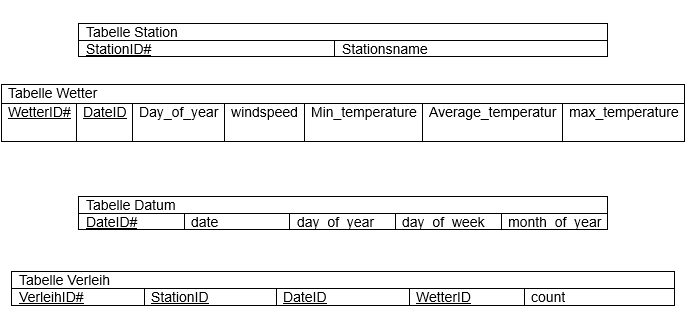
\includegraphics[width=\textwidth]{datenbankschema[1].png}
    \caption{Hier haben wir ein Datenbank-Schema in der 1. und 2. Normalform erstellt. Da sich die Daten bereits in der 1. Normalform befunden haben, mussten wir nichts weiter ändern. Schlüsselattribute sind mit \# gekennzeichnet, Primärschlüssel sind unterstrichen.}
    \label{fig:datenbankschema}
\end{figure}

\newpage 

\newpage 



\label{sec:datenbank-schema}

\subsection{Create Table - Tabellen erstellen}
\label{sec:create-table}

Mit \texttt{CREATE TABLE} erstellen wir unsere 4 Tabellen. Wichtig dabei ist, dass wir immer den richtigen Datentyp wählen (\texttt{int}, \texttt{text}, \texttt{real}) und den Primärschlüssel mit \texttt{PRIMARY KEY} benennen.

\begin{figure}[h!]
    \centering
    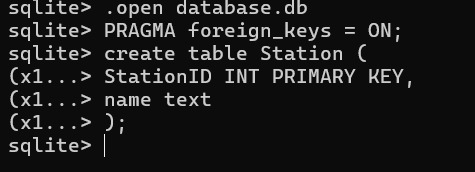
\includegraphics[width=0.9\textwidth]{Nummer 1.jpg}
    \caption{Tabelle Station: Definition mit \texttt{CREATE TABLE}}
    \label{fig:table-station}
\end{figure}

\begin{figure}[h!]
    \centering
    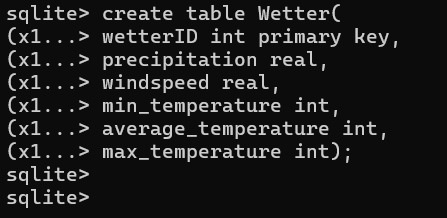
\includegraphics[width=0.9\textwidth]{Nummer 2.jpg}
    \caption{Tabelle Wetter: Definition mit \texttt{CREATE TABLE}}
    \label{fig:table-wetter}
\end{figure}

\begin{figure}[h!]
    \centering
    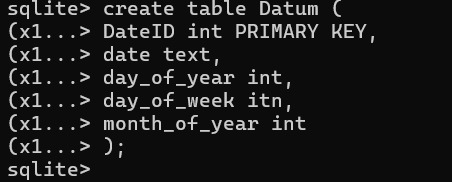
\includegraphics[width=0.9\textwidth]{Nummer 3.jpg}
    \caption{Tabelle Datum: Definition mit \texttt{CREATE TABLE}}
    \label{fig:table-datum}
\end{figure}

\begin{figure}[h!]
    \centering
    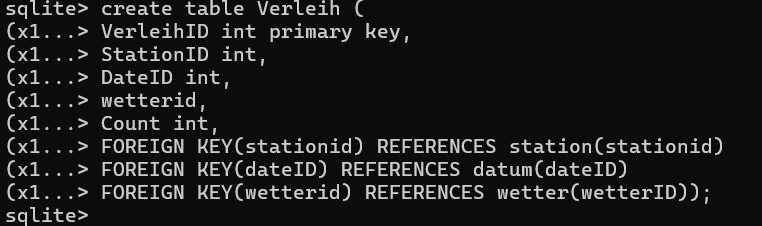
\includegraphics[width=0.9\textwidth]{Nummer 4.jpg}
    \caption{Tabelle Verleih: Definition mit \texttt{CREATE TABLE} und Fremdschlüssel}
    \label{fig:table-verleih}
\end{figure}

\newpage
\newpage 

\subsection{Importieren von Daten in SQLite}
\label{sec:sqlite-import}

In SQLite können wir nun durch die folgenden Befehle:

\begin{verbatim}
.mode csv
.import stationen.csv station
\end{verbatim}

die Daten in unsere Tabelle \texttt{Station} importieren. \texttt{Stationen.csv} ist dabei der Dateiname mit den Daten für die Tabelle, und \texttt{station} ist die zuvor erstellte Tabelle. Wichtig ist zu beachten, dass die CSV-Datei und SQLite3 im selben Ordner liegen, da ansonsten der Dateipfad angegeben werden muss.

Zusätzlich können die restlichen Tabellen mit den folgenden Befehlen importiert werden:

\begin{verbatim}
.mode csv
.separator ;
.import stationenneu.csv station
.import wetter.csv wetter
.import datum.csv datum
.import verleih.csv verleih
\end{verbatim}

\newpage 
\newpage 

\subsection{Abfrage der höchsten mittleren Temperatur}
\label{sec:highest-temp-query}

Um die höchste mittlere Temperatur in Grad Celsius abzufragen, können wir den folgenden Code nutzen:

\begin{verbatim}
.mode column
.headers on

Select max((average_temperature - 32) * 5.0 / 9) 
    AS HoechsteDurchschnittstemperatur_Celsius
from wetter;
\end{verbatim}

\begin{figure}[h!]
    \centering
    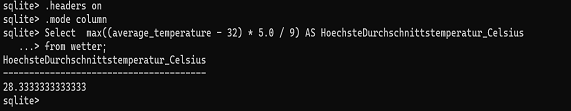
\includegraphics[width=0.9\textwidth]{letztes b.png}
    \caption{Abfrage der höchsten mittleren Temperatur in SQLite}
    \label{fig:highest-temp-query}
\end{figure}

\newpage 


\section*{Literatur}
\begin{itemize}
    \item \hypertarget{litref}{[1]} Achim Klenke. \textit{Wahrscheinlichkeitstheorie}. Springer, 3. Auflage, 2013.
    \item \textbf{Repository-Link:} \url{https://github.com/Envvas/Latex_code}
\end{itemize}

\end{document}
